\documentclass[../notes.tex]{subfiles}

\pagestyle{main}
\renewcommand{\chaptermark}[1]{\markboth{\chaptername\ \thechapter\ (#1)}{}}
\setcounter{chapter}{11}

\begin{document}




\chapter{Experimental Kinetics}
\section{Kinetics of Catalytic Reactions}
\begin{itemize}
    \item \marginnote{11/19:}Last week's lectures.
    \begin{itemize}
        \item Very simple kinetic scenarios.
        \item Linearizations allows us to extract essential kinetic parameters for reactions.
        \item Kinetic descriptions for multistep processes.
        \item Steady-state approximation, quasi-equilibrium approximation.
    \end{itemize}
    \item Today: Kinetics of Catalytic Reactions.
    \item Catalysts speed up the rate of reaction without altering the thermodynamics.
    \item Consider the following balanced chemical reaction.
    \begin{equation*}
        \ce{A + B + cat -> P + cat}
        \qquad\equiv\qquad
        \ce{A + B ->[cat] P}
    \end{equation*}
    \begin{itemize}
        \item Since the catalyst appears on both sides of the reaction, we typically write it over the arrow.
        \item This notational simplification alides a great deal of multistep complexity.
    \end{itemize}
    \item Consider a hypothetical potential energy surface.
    \begin{figure}[h!]
        \centering
        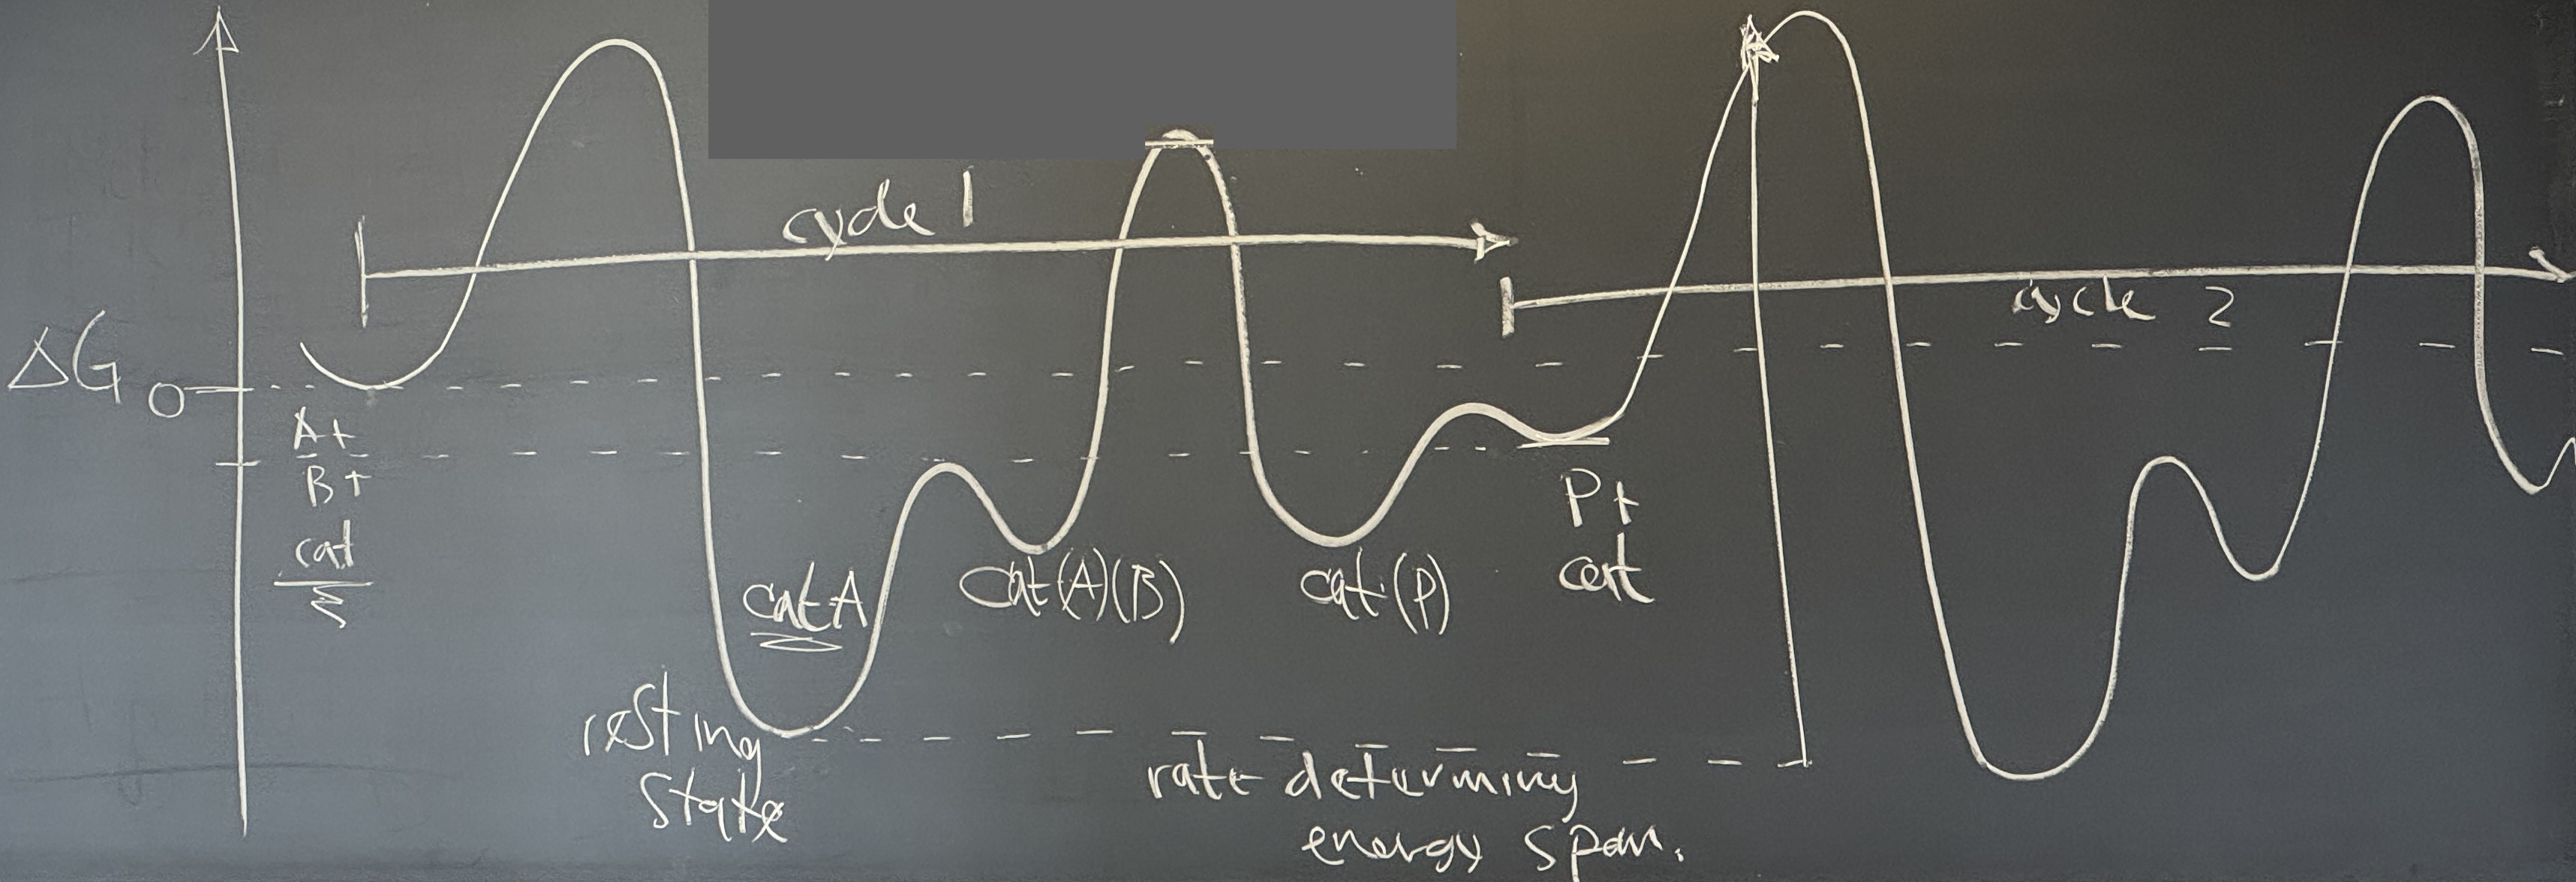
\includegraphics[width=0.8\linewidth]{modelCatPES.JPG}
        \caption{Model catalytic potential energy surface.}
        \label{fig:modelCatPES}
    \end{figure}
    \begin{itemize}
        \item Define a reference energy as zero; suppose the starting materials (\ce{A + B + cat}) begin here.
        \item Suppose, then, that they proceed through a multistep potential energy surface along our reaction coordinate.
        \item If this were a stoichiometric reaction, the first step would be rate-determining (highest energy barrier), and the first intermediate would be the product (lowest energy species).
        \begin{itemize}
            \item But we're catalytic, so we have to consider cycles 2, 3, \dots
            \item These cycles are driven forward by the ever-so-slight difference in energy $\Delta G$ between starting materials and products.
        \end{itemize}
        \item The "first intermediate" is actually the catalyst \textbf{resting state}.
        \begin{itemize}
            \item Indeed, the thing that we throw in may not be the dominant species in solution!
            \item It could be \ce{cat*(A)}, \ce{cat*(A)(B)}, or \ce{cat*(P)}!
        \end{itemize}
        \item Similarly, the difference in energy between the lowest valley and highest peak is the \textbf{rate-determining energy span}.
        \item Reference (good description of rate-determining energy span): \textcite{bib:modelCatPES}.
    \end{itemize}
    \item Because continuous potential energy surfaces are not great representations, we typically view catalysts as acting in \textbf{catalytic cycles}.
    \begin{figure}[h!]
        \centering
        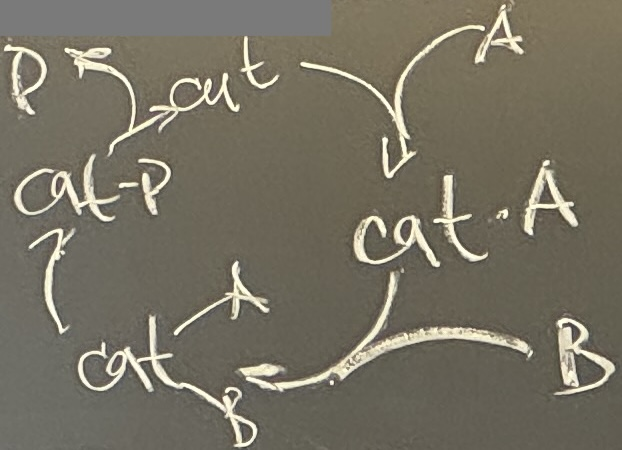
\includegraphics[width=0.23\linewidth]{modelCatCycle.JPG}
        \caption{Model catalytic cycle.}
        \label{fig:modelCatCycle}
    \end{figure}
    \begin{itemize}
        \item This is not that uncommon a catalytic cycle to find!
    \end{itemize}
    \item Let's now do a kinetic analysis of this model catalytic cycle, using some of the tools developed last lecture.
    \begin{figure}[h!]
        \centering
        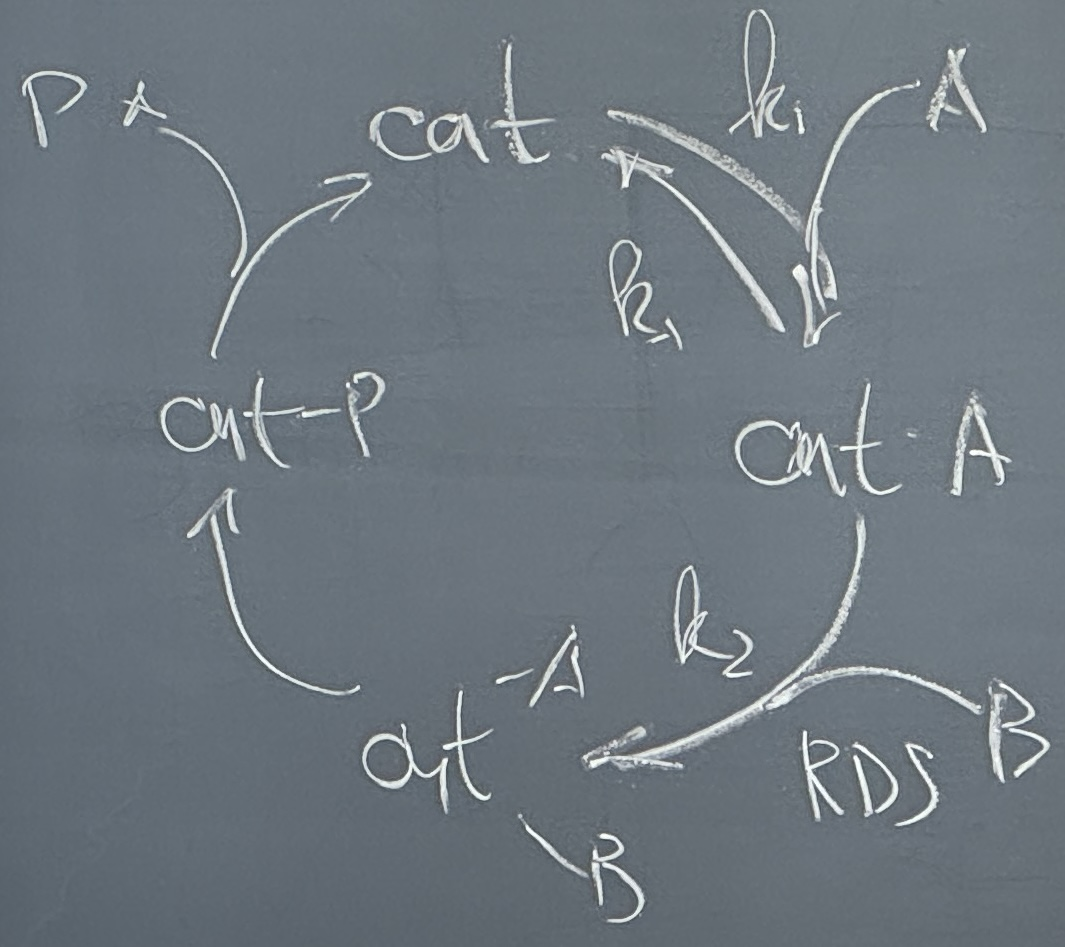
\includegraphics[width=0.3\linewidth]{modelCatCycleKin.JPG}
        \caption{Model catalytic cycle (kinetic analysis).}
        \label{fig:modelCatCycleKin}
    \end{figure}
    \begin{itemize}
        \item Assume that the first step is a reversible binding to \ce{A}.
        \item Recall that the rate-determining step follows the resting state. Thus,
        \begin{equation*}
            \rate = \dv{\cnc{P}}{t}
            = -\dv{\cnc{A}}{t}
            = k_2\cnc{cat*A}\cnc{B}
        \end{equation*}
        \item We can then apply our rule of thumb for the steady-state approximation.
        \begin{equation*}
            \rate = \frac{k_1k_2\cnc{A}\cnc{B}\cnc{cat}}{k_{-1}+k_2\cnc{B}}
        \end{equation*}
    \end{itemize}
    \item Going forward, it will be useful to define the total concentration of catalyst
    \begin{equation*}
        \cnc[T]{cat} := \cnc{cat}+\cnc{cat*A}+\cnc{cat*AB}+\cnc{cat*P}
    \end{equation*}
    \begin{itemize}
        \item To derive the rate law for Figure \ref{fig:modelCatCycleKin} in terms of $\cnc[T]{cat}$ --- an observable --- we'd need a system of equations.
    \end{itemize}
    \item Let's now consider a different (simpler) catalytic cycle to develop some core ideas.
    \begin{figure}[h!]
        \centering
        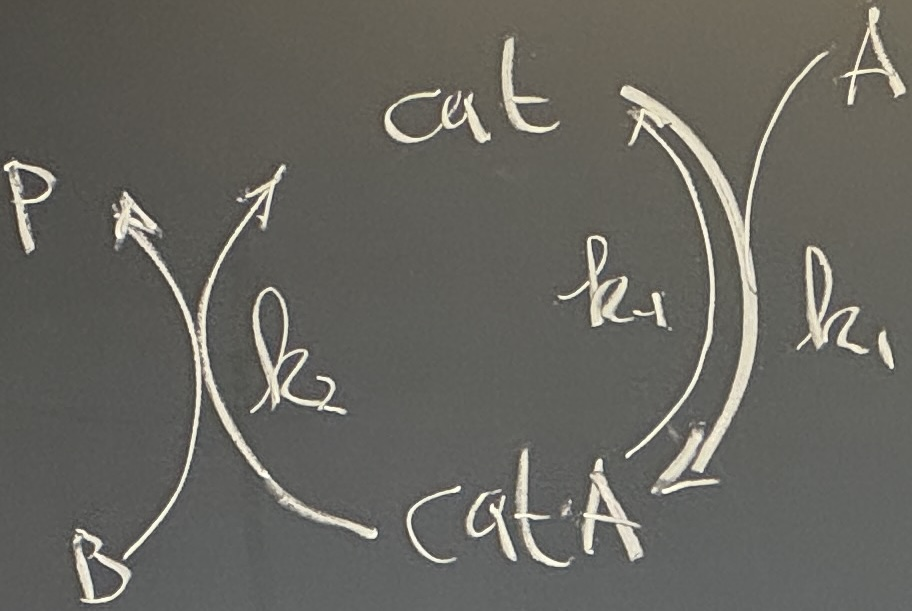
\includegraphics[width=0.23\linewidth]{modelCat2Kin.JPG}
        \caption{Model two-step catalytic cycle (kinetic analysis).}
        \label{fig:modelCat2Kin}
    \end{figure}
    \begin{itemize}
        \item This cycle pertains to a reaction
        \begin{equation*}
            \ce{A + B ->[cat] P}
        \end{equation*}
        \item If the second step is rate-determining, then
        \begin{equation*}
            \rate = k_2\cnc{cat*A}\cnc{B}
        \end{equation*}
        \item It will also be useful to have the assumption
        \begin{equation*}
            \cnc[T]{cat} = \cnc{cat}+\cnc{cat*A}
        \end{equation*}
    \end{itemize}
    \item Let's now evaluate this catalytic cycle using the quasi-equilibrium assumption.
    \begin{itemize}
        \item Warning: Lots of algebra coming up!
        \begin{itemize}
            \item Squiggly lines on the board mean abbreviations.
        \end{itemize}
        \item The quasi-equilibrium assumption tells us that
        \begin{equation*}
            K = \frac{k_1}{k_{-1}}
            = \frac{\cnc{cat*A}}{\cnc{cat}\cnc{A}}
        \end{equation*}
        \item We first solve for the concentration of the catalyst.
        \begin{equation*}
            \cnc{cat} = \frac{\cnc{cat*A}}{K\cnc{A}}
        \end{equation*}
        \item We can drop this into our expression for the total catalyst.
        \begin{equation*}
            \cnc[T]{cat} = \frac{\cnc{cat*A}}{K\cnc{A}}+\cnc{cat*A}
        \end{equation*}
        \item We can factor out the $\cnc{cat*A}$'s.
        \begin{equation*}
            \cnc[T]{cat} = \cnc{cat*A}\left( \frac{1}{K\cnc{A}}+1 \right)
        \end{equation*}
        \item Rearrange this to solve for $\cnc{cat*A}$.
        \begin{equation*}
            \cnc{cat*A} = \frac{\cnc[T]{cat}}{1/K\cnc{A}+1}
        \end{equation*}
        \item Remove this fractional denominator via multiplication by a clever form of 1 (namely, $K\cnc{A}/K\cnc{A}$).
        \begin{equation*}
            \cnc{cat*A} = \frac{K\cnc{A}\cnc[T]{cat}}{1+K\cnc{A}}
        \end{equation*}
        \item We can now drop this back into the rate expression to get an expression for the rate in terms of the overall catalyst concentration, which is more useful because that's an observable (we know how much we put in!).
        \begin{equation*}
            \rate = \frac{k_2K\cnc{A}\cnc{B}\cnc[T]{cat}}{1+K\cnc{A}}
        \end{equation*}
        \item Note that we could also write the $K$'s above as $\Keq$'s.
    \end{itemize}
    \item Let's now derive an analogous expression for the catalytic cycle in Figure \ref{fig:modelCat2Kin}, but this time under the steady-state approximation.
    \begin{itemize}
        \item We initially obtain
        \begin{equation*}
            \cnc{cat*A} = \frac{k_1\cnc{A}\cnc{cat}}{k_{-1}+k_2\cnc{B}}
        \end{equation*}
        \item Rearranging yields
        \begin{equation*}
            \cnc{cat} = \frac{\cnc{cat*A}(k_{-1}+k_2\cnc{B})}{k_1\cnc{A}}
        \end{equation*}
        \item Using the fact that $\cnc{cat}=\cnc[T]{cat}-\cnc{cat*A}$, we obtain
        \begin{equation*}
            \frac{\cnc{cat*A}(k_{-1}+k_2\cnc{B})}{k_1\cnc{A}} = \cnc[T]{cat}-\cnc{cat*A}
        \end{equation*}
        \item We get rid of the denominator by multiplying both sides by $k_1\cnc{A}$, collect a couple of terms, and rearrange into
        \begin{equation*}
            \cnc{cat*A}(k_1\cnc{A}+k_{-1}+k_2\cnc{B}) = k_1\cnc{A}\cnc[T]{cat}
        \end{equation*}
        \item Then divide both sides by the term in parentheses on the left.
        \begin{equation*}
            \cnc{cat*A} = \frac{k_1\cnc{A}\cnc[T]{cat}}{k_1\cnc{A}+k_{-1}+k_2\cnc{B}}
        \end{equation*}
        \item This substitution can now be dropped back into our rate law.
        \begin{align*}
            \rate &= k_2\cnc{cat*A}\cnc{B}\\
            &= \frac{k_1k_2\cnc{A}\cnc{B}\cnc[T]{cat}}{k_{-1}+k_2\cnc{B}+k_1\cnc{A}}
        \end{align*}
        \item We now multiply by another clever form of 1 (namely the inverse of $k_{-1}$ on both top and bottom).
        \begin{equation*}
            \rate = \frac{\frac{k_1}{k_{-1}}k_2\cnc{A}\cnc{B}\cnc[T]{cat}}{1+\frac{k_2}{k_{-1}}\cnc{B}+\frac{k_1}{k_{-1}}\cnc{A}}
        \end{equation*}
        \begin{itemize}
            \item This is known as the \textbf{one plus rate form} of the rate law because of the "$1+$" in the denominator.
        \end{itemize}
    \end{itemize}
    \item We can now compare the two rate laws we've derived.
    \begin{itemize}
        \item We do this by assuming that $k_{-1}\gg k_2$, which is exactly the scenario in which the quasi-equilibrium assumption would apply!
        \item We approach a limit where we can ignore the $k_2/k_{-1}$ term in the denominator, and $k_1/k_{-1}=\Keq$ (as established previously).
    \end{itemize}
    \item Let's consider some limiting scenarios.
    \begin{itemize}
        \item This will help us partially eliminate complexity.
        \item First, let's consider the scenario in which
        \begin{equation*}
            1 \gg \frac{k_2}{k_{-1}}\cnc{B} \approx \frac{k_1}{k_{-1}}\cnc{A}
        \end{equation*}
        \begin{itemize}
            \item In this case, the denominator vanishes and the simplified rate law is
            \begin{equation*}
                \rate = \frac{k_1}{k_{-1}}\cnc{A}\cnc{B}\cnc[T]{cat}
            \end{equation*}
            \item Since this constraint implies that $k_{-1}\gg k_2$, the second step must be rate-determining.
            \item It also follows that $\cnc[T]{cat}\approx\cnc{cat}$, and hence the resting state of the catalyst is the unbound catalyst!
            \item We can also say that the second step is \textbf{turnover-limiting}.
        \end{itemize}
        \item Second, let's consider the scenario in which
        \begin{equation*}
            \frac{k_2}{k_{-1}}\cnc{B} \gg \text{others}
        \end{equation*}
        \begin{itemize}
            \item By "others," we mean the other two terms in the denominator.
            \item In this case, the simplified rate law is
            \begin{equation*}
                \rate = k_1\cnc{A}\cnc[T]{cat}
            \end{equation*}
            \item This constraint implies that the first step is rate-determining.
            \item Hence, the reaction with \ce{B} (zero-order) is post-rate limiting.
            \item It follows additionally that once again, the resting state of the catalyst is the unbound catalyst!
        \end{itemize}
        \item Third, let's consider the scenario in which
        \begin{equation*}
            \frac{k_1}{k_{-1}}\cnc{A} \gg \text{others}
        \end{equation*}
        \begin{itemize}
            \item In this case, the simplified rate law is
            \begin{equation*}
                \rate = k_2\cnc{B}\cnc[T]{cat}
            \end{equation*}
            \item Zero-order dependence on $\cnc{A}$ implies that the catalyst is fully saturated with $\cnc{A}$.
            \item Hence, the second step is rate-determining and the resting state is the bound catalyst.
        \end{itemize}
        \item Fourth, everything matters.
        \begin{itemize}
            \item This scenario is not limiting but is, unfortunately, common.
            \item This implies a kinetic pathway in which all species are at roughly similar energies with roughly similar transition structures.
            \item This is often a good thing for catalysis, but we'll get there.
        \end{itemize}
    \end{itemize}
    \item Aside: The one plus rate form.
    \begin{equation*}
        \rate = \frac{c_1\cnc{A}\cnc{B}\cnc[T]{cat}}{1+c_2\cnc{A}+c_3\cnc{A}\cnc{B}+c_4\cnc{P}}
    \end{equation*}
    \begin{itemize}
        \item The rate law takes on the above general structure.
        \item We have a constant (the "kinetic term") $c$ modified by the concentrations of the inputs in the numerator, collectively referred to as the potential terms (because they reflect something about the TST with respect to the ground state).
        \item The denominator --- the \textbf{adsorption term} --- consists of all the forms that the catalyst can take.
        \item What do the constants tell us?
        \begin{itemize}
            \item $c_1$ tells us about the naked catalyst.
            \item $c_2\cnc{A}$ can tell us about the \ce{cat*A} complex.
            \item $c_3\cnc{A}\cnc{B}$ can tell us about the \ce{cat*AB} complex.
            \item $c_4\cnc{P}$ can tell us about the \ce{cat*P} complex.
        \end{itemize}
        \item Goal of this exercise: Gain intution for the algebra.
        \begin{itemize}
            \item The best kineticists can easily see the chemistry in rate laws the way that most organic chemists can see it in Lewis structures.
            \begin{itemize}
                \item Donna Blackmond at Scripps is one of Alex's favorite kineticists.
            \end{itemize}
            \item Similarly, spectroscopists can see chemistry in derivative waveforms; "what a power to have!"
        \end{itemize}
    \end{itemize}
    \item How do we increase the rate, i.e., max out the rate law?
    \begin{itemize}
        \item We want to get the denominator to go away.
        \item This gives Scenario 3, in which all of the substrate is bound to the catalyst and it's doing it's thing as fast as it can.\footnote{Why should this scenario give the fastest rate??}
        \begin{equation*}
            \rate_\text{max} = k_2\cnc{B}\cnc[T]{cat}
        \end{equation*}
    \end{itemize}
    \item Let's plop $\rate_\text{max}$ into our steady-state approximation rate law, and multiply it by $1=k_{-1}/k_{-1}$.
    \begin{equation*}
        \rate = \frac{\rate_\text{max}k_1\cnc{A}}{k_{-1}+k_2\cnc{B}+k_1\cnc{A}}
    \end{equation*}
    \begin{itemize}
        \item Now define
        \begin{equation*}
            \frac{1}{K_m} = \frac{k_1}{k_{-1}+k_2\cnc{B}}
        \end{equation*}
        \item It follows that
        \begin{equation*}
            \rate = \frac{\rate_\text{max}\cnc{A}}{K_m+\cnc{A}}
        \end{equation*}
    \end{itemize}
    \item Under the quasi-equilibrium assumption, we can assume something else.
    \begin{equation*}
        \rate = \frac{\rate_\text{max}\Keq\cnc{A}}{1+\Keq\cnc{A}}
    \end{equation*}
    \begin{itemize}
        \item Now define
        \begin{equation*}
            K_D = \frac{1}{\Keq}
        \end{equation*}
        as the dissociation constant for the \ce{cat*A} complex.
        \item It follows that
        \begin{equation*}
            \rate = \frac{\rate_\text{max}\cnc{A}}{K_D+\cnc{A}}
        \end{equation*}
    \end{itemize}
    \item $K_m$ takes us into \textbf{Michaelis-Menten kinetics}.
    \begin{itemize}
        \item Defined in the early twentieth century to guide our emerging understanding of biochemical kinetics.
        \item Using the historical nomenclature (substrate and enzyme), we have
        \begin{equation*}
            \ce{S + E <=>[$k_f$][$k_r$] S*E ->[$k_\text{cat}$] P}
        \end{equation*}
        \item There is a relationship here to saturation kinetics, defined in the limiting scenarios with Figure \ref{fig:modelCat2Kin}.
        \item Michaelis and Menten talked about a kinetic velocity $v_\text{max}$ where we go from asymptotic speed down to a first-order dependence on $\cnc{S}$.
        \item Other relevant expressions:
        \begin{align*}
            K_m &= \frac{k_r+k_\text{cat}}{k_f}&
            v &= \frac{v_\text{max}\cnc{S}}{K_m+\cnc{S}}
        \end{align*}
        \item If $K_m=\cnc{S}$, then $v=v_\text{max}/2$.
        \item We can experimentally determine the Michaelis constant by assaying a bunch of different initial rates at different concentrations.
    \end{itemize}
    \item What's the point of Michaelis-Menten kinetics?
    \begin{figure}[h!]
        \centering
        \begin{subfigure}[b]{0.4\linewidth}
            \centering
            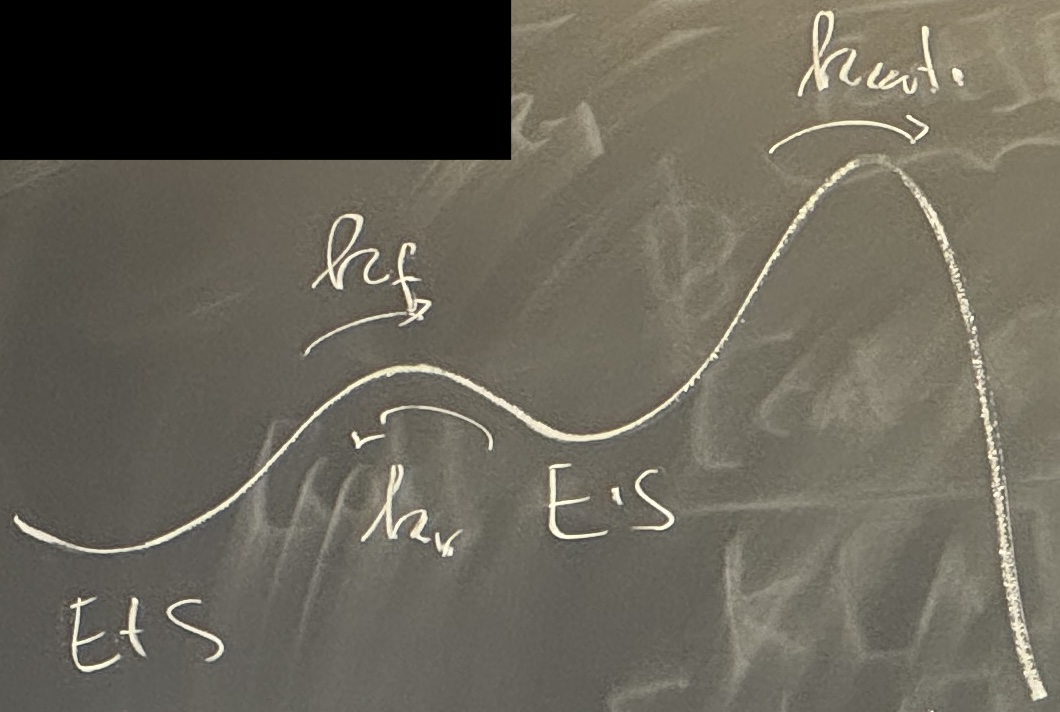
\includegraphics[width=0.8\linewidth]{MMkina.JPG}
            \caption{Zeroeth-order.}
            \label{fig:MMkina}
        \end{subfigure}
        \begin{subfigure}[b]{0.4\linewidth}
            \centering
            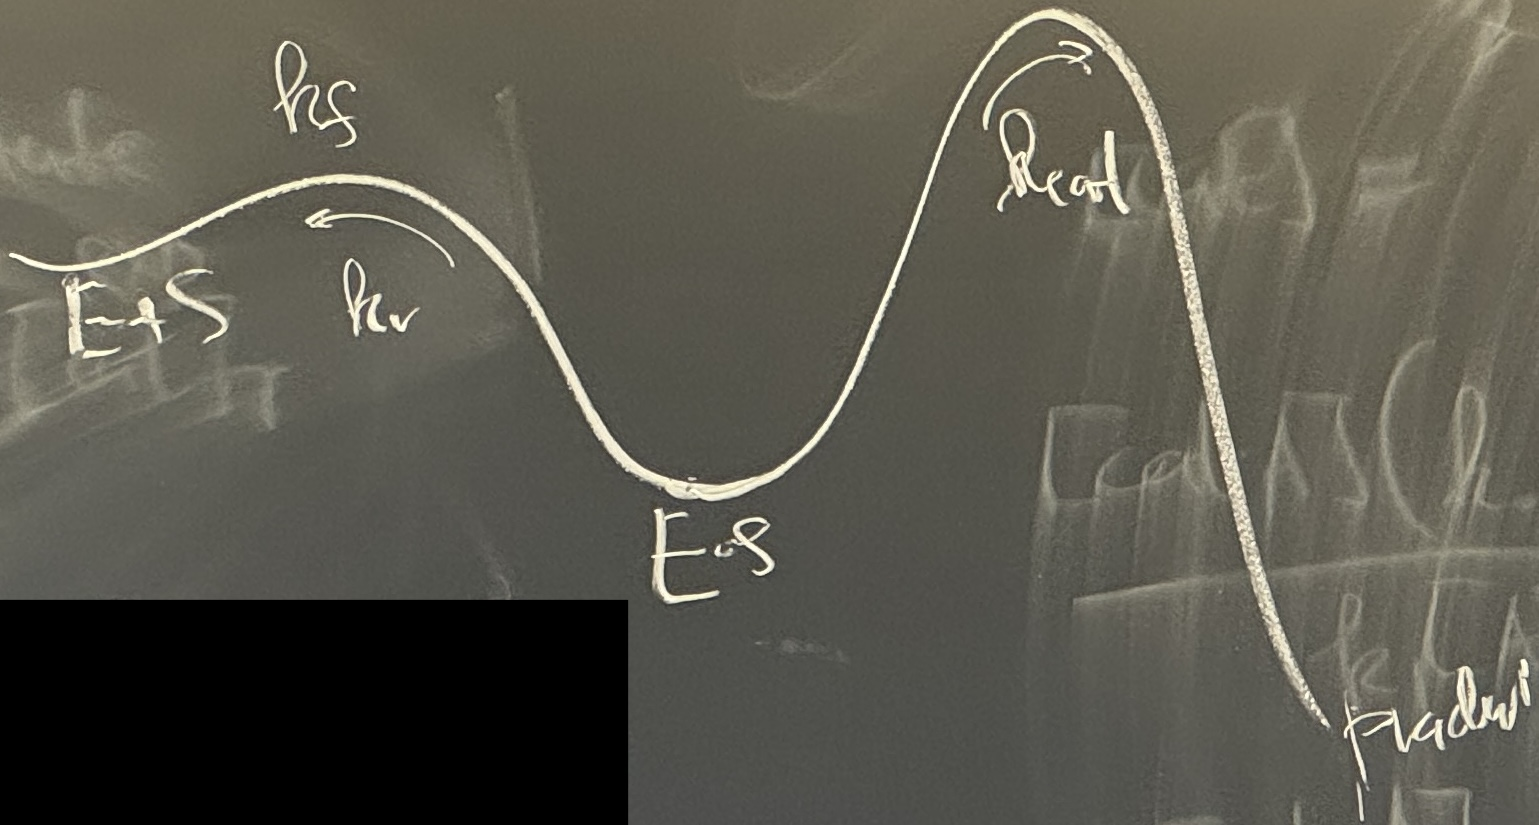
\includegraphics[width=0.95\linewidth]{MMkinb.JPG}
            \caption{First-order.}
            \label{fig:MMkinb}
        \end{subfigure}
        \caption{Michaelis-Menten kinetic regimes.}
        \label{fig:MMkin}
    \end{figure}
    \begin{itemize}
        \item Enzymes can be characterized according the Michaelis constant $K_m$ and the intrinsic rate constant $k_\text{cat}$.
        \item When we're zeroeth order in the substrate, we have one kinetic regime.
        \item When we're first-order in the substrate, we have a kinetic regime that's more like quasi-equilibrium!
        \item How well the enzyme binds the substrate is a measure of how efficient the catalyst is.
    \end{itemize}
    \item When $k_r\gg k_\text{cat}$,
    \begin{equation*}
        K_m \approx \frac{k_r}{k_f} = K_D
    \end{equation*}
    \begin{itemize}
        \item This ratio measures how well the enzyme binds to the substrate.
    \end{itemize}
    \item When $k_\text{cat}\gg k_r$,
    \begin{equation*}
        K_m \approx \frac{k_\text{cat}}{K_m} =: \text{specificity constant}
    \end{equation*}
    \begin{itemize}
        \item These ratios can be analyzed as the specificity constant for a specific enzyme.
        \item Describes an enzyme's preference (both in terms of binding and reactivity) for one substrate over another.
    \end{itemize}
    \item Example: Fumerase (responsible for redox transport).
    \begin{itemize}
        \item $K_m=\num{5e-6}$, and $k_\text{cat}=\num{8e2}$, so SC is $\num{e7}$.
    \end{itemize}
    \item Example: Carbonic anhydrase.
    \begin{itemize}
        \item $K_m=\num{2.6e-2}$, and $k_\text{cat}=\num{4e5}$, so SC is $\num{e8}$.
    \end{itemize}
    \item So for great catalysis, you want the catalyst to find substrate quickly and immediately turn it over.
    \begin{itemize}
        \item These two catalysts operate near the diffusion limit (which is ideal); they are near-perfect.
    \end{itemize}
    \item References.
    \begin{itemize}
        \item \textcite{bib:EnzymeCat}.
        \item A beautiful piece of literature; the touchstone for biological catalysis, per Alex.
    \end{itemize}
\end{itemize}



\section{Techniques for Kinetics Determinations}
\begin{itemize}
    \item \marginnote{11/21:}Today: Experimental techniques for kinetic determination.
    \begin{itemize}
        \item In contrast to last time's algebra, we'll figure out today that many of those algebraic techniques were unnecessary.
        \item Many techniques of kinetic analysis can be done with just a few observational experiments.
        \item Goal of today: Convince us that kinetic analysis can be easy\dots and even fun!
    \end{itemize}
    \item Consider the following reaction from last time.
    \begin{equation*}
        \ce{A + B ->[cat] P}
    \end{equation*}
    \begin{itemize}
        \item Recall from last time that kinetics can be used to elucidate the transition state structure.
        \item Recall from last week that linearizing data can give us the reaction order.
        \item However, we can access rate constant data without regression by using the \textbf{method of initial rates}.
    \end{itemize}
    \item \textbf{Method of initial rates}: Assume that $\rate=k\cnc{A}^a\cnc{B}^b\cnc{cat}^c$, take time courses, and make plots as in Figure \ref{fig:kAB2} to extract $k$.
    \begin{figure}[h!]
        \centering
        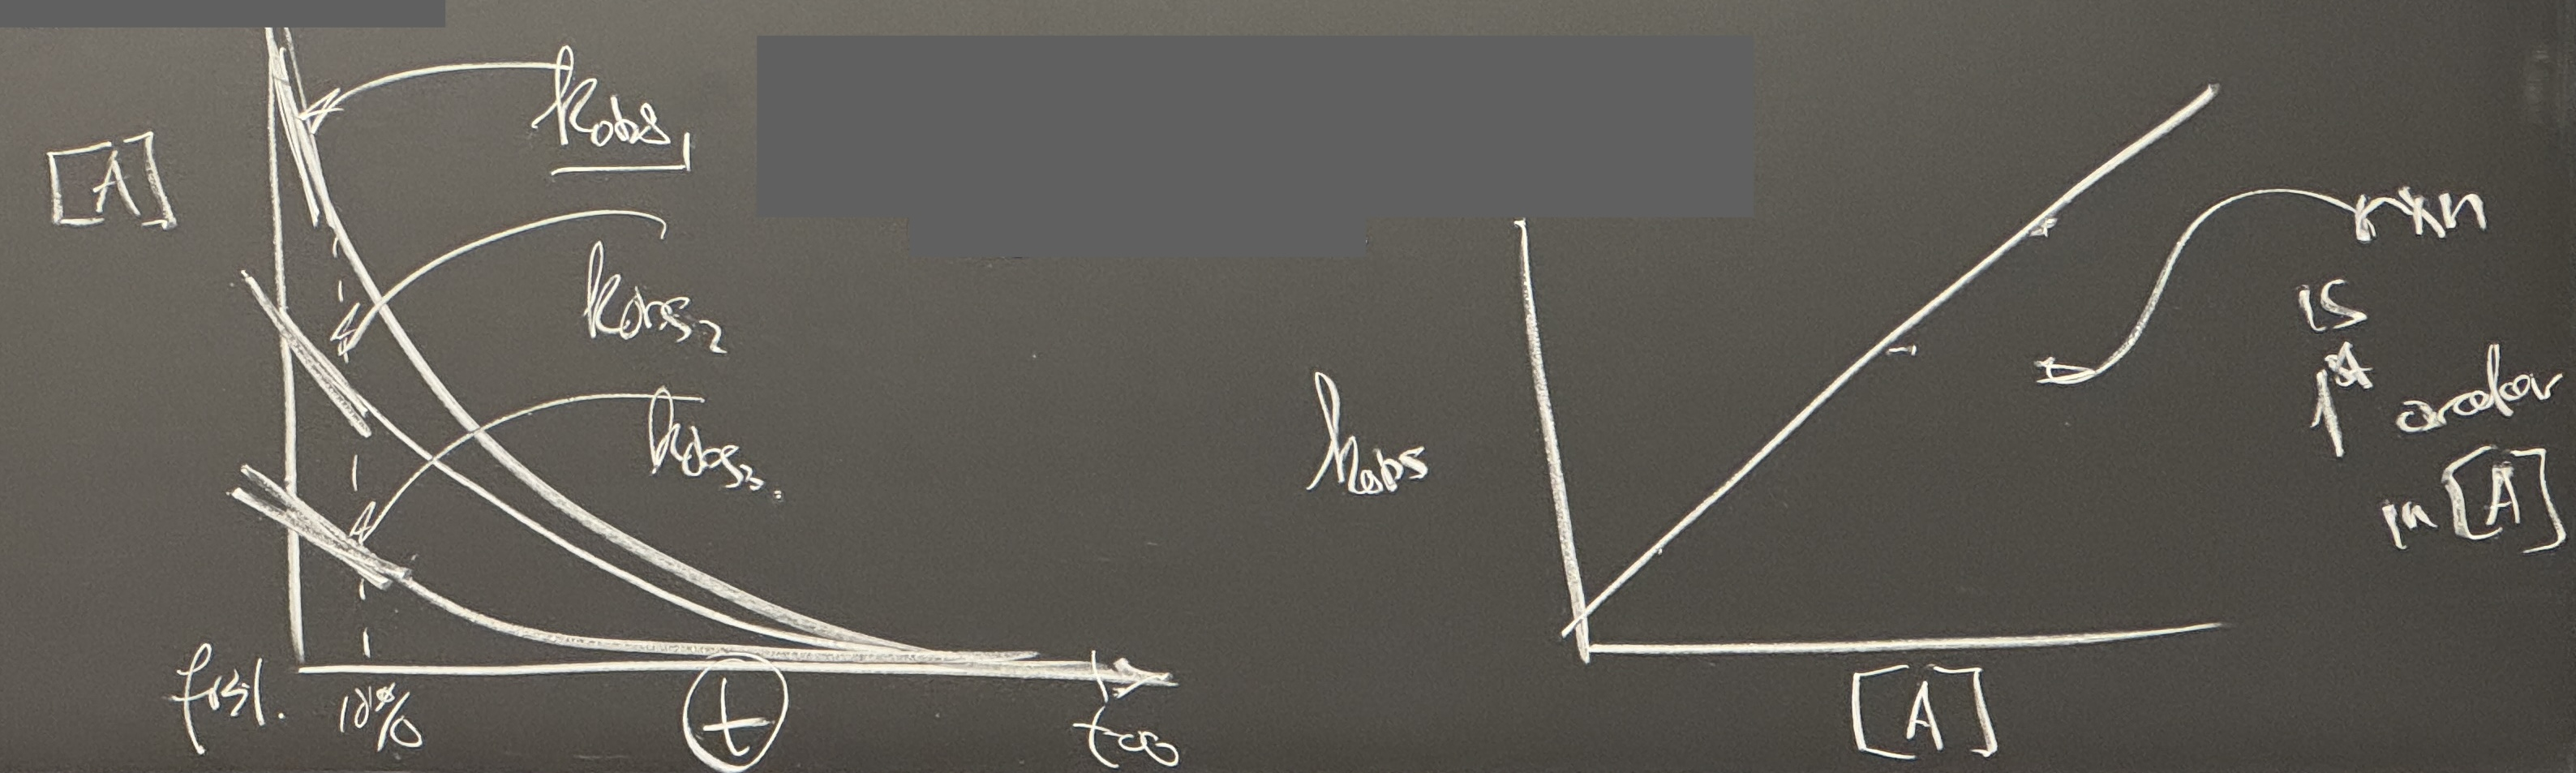
\includegraphics[width=0.75\linewidth]{methodInitRate.JPG}
        \caption{Method of initial rates.}
        \label{fig:methodInitRate}
    \end{figure}
    \begin{itemize}
        \item Begin by taking a time course for $\cnc{A}$.
        \item We can extract $\kobs$ from initial slopes
        \begin{equation*}
            -\dv{\cnc{A}}{t} = \dv{\cnc{P}}{t} = \kobs
        \end{equation*}
        if we're in a regime where all of the other concentrations are basically constant.
        \item If we consider the first, say, 10\% of the reaction, then this approximate initial slope gives us $\kobs$ directly.
        \item We can vary the initial concentration of $\cnc{A}$ to get multiple values of $\kobs$.
        \item Then --- as in Figure \ref{fig:kAB2} --- we can plot $\kobs$ vs. $\cnc{A}$ to learn the order of our reaction.
    \end{itemize}
    \item The time domain matters a lot.
    \begin{itemize}
        \item If $t\in[\SI{e2}{\second},\SI{e6}{\second}]$, we're in the "conventional" range for reaction speed.
        \begin{itemize}
            \item Techniques like NMR are applicable here. These can allows us to assign concentration and structure in one experiment.
            \item UV-Vis can also be good here.
            \item FT-IR is also nice; it's very fast.
            \item GC-MS is another recommended one in the conventional time domain.
        \end{itemize}
        \item If $t\in[\SI{e-3}{\second},\SI{e1}{\second}]$, our reactions are too fast to pull out an aliquot.
        \begin{itemize}
            \item As such, we need stopped flow kinetics.
        \end{itemize}
        \item If $t\in[\SI{e-12}{\second},\SI{e-6}{\second}]$, our reactions are too fast for mechanical injection into a compartment.
        \begin{itemize}
            \item As such, use \textbf{flash photolysis}: Flash a light and follow the course with (typically) UV-Vis.
        \end{itemize}
    \end{itemize}
    \item How can we directly read out rate data from a reaction?
    \begin{itemize}
        \item Calorimetry: The flow of heat from the vessel is directly related to the rate.
        \item Mass transport and gas flow: Also good direct measurements.
    \end{itemize}
    \item Usefulness of the method of initial rates.
    \begin{itemize}
        \item Pros.
        \begin{itemize}
            \item No complex math.
            \item Direct access to $\kobs$.
            \item Easy.
            \begin{itemize}
                \item You've already got the starting materials, so just set up one more reaction!
            \end{itemize}
            \item Useful for trickier reactions with more complex kinetic scenarios, e.g., heterogeneous catalysis.
        \end{itemize}
        \item Cons.
        \begin{itemize}
            \item Prone to error ($\pm 10\%$ at best).
            \begin{itemize}
                \item We've got only a few data points from a short window in which not much has happened.
            \end{itemize}
            \item The first 10\% of the reaction course may not be representative of the entire reaction.
            \begin{itemize}
                \item In fact, there are many cases where the first 10\% is patently \emph{not} representative of the entire reaction (see Figure \ref{fig:complexTimecourse}).
                \item Example: A burst of speed at the very beginning due, for example, to a catalyst turning over very quickly because there's a large amount of it unbound early on.
                \item Example: An \textbf{induction period} before the reaction begins in earnest.
            \end{itemize}
            \item Can be labor intensive.
            \begin{itemize}
                \item We need several measurements of $\kobs$; two measurements define a straight line, technically, but at least three are needed to be experimentally viable.
            \end{itemize}
        \end{itemize}
    \end{itemize}
    \item Alex has personally done such initial rate experiments, despite the difficulties. But in the computer age, the method of initial rates has been outpaced by \textbf{whole-reaction kinetics}.
    \begin{itemize}
        \item We can take a bunch of data points, and the computer can just fit it to a curve.
        \item We can then transform this into a linear plot of $\dv*{\cnc{A}}{t}$ vs. $\cnc{A}$.
        \item Curve fitting via polynomial regression: Fit
        \begin{equation*}
            \cnc[$t$]{A} = f(t) = a+bt+ct^2+dt^3+et^4+ft^5+\cdots
        \end{equation*}
        \begin{itemize}
            \item If we have enough terms, we can fit basically anything!
            \item And then polynomials are nice because they're easily differentiated.
        \end{itemize}
        \item Computers can do all this.
    \end{itemize}
    \item How can we account for saturation kinetics?
    \begin{itemize}
        \item Recall that as $\cnc{A}$ decreases, we sometimes switch kinetic regimes.
        \begin{itemize}
            \item Such data may be hard to manipulate via linear regression.
            \item This can be easier to look at on a rate vs. concentration plot than a concentration vs. time plot.
        \end{itemize}
        \item Note that on a rate vs. concentration plot, reactions with induction periods show up as humps.
        \begin{itemize}
            \item This is because the reaction takes a bit to get going (i.e., during the induction period), then accelerates to normal, and then tapers off.
            \item We can still polynomial fit these!
        \end{itemize}
    \end{itemize}
    \item Experimental chemistry offers all manner of complex kinetics, not just simple integrated rate laws.
    \begin{itemize}
        \item So we need powerful techniques.
    \end{itemize}
    \item To solve these challenges, use reaction progress kinetic analysis (RPKA).
    \begin{itemize}
        \item Developed by Donna Blackmond (Scripps) --- a modern genius of reaction kinetics.
        \item She has a few valuable, albeit impenetrable, pieces of literature.
        \begin{itemize}
            \item \textcite{bib:RPKA1}.
            \item \textcite{bib:RPKA2}.
        \end{itemize}
        \item This method does not shoehorn reactions into models that they don't fit.
        \item Two relevant techniques.
        \begin{itemize}
            \item Same excess experiment.
            \item Different excess experiment.
        \end{itemize}
    \end{itemize}
    \item Same excess experiment.
    \begin{figure}[h!]
        \centering
        \begin{subfigure}[b]{0.4\linewidth}
            \centering
            \begin{tikzpicture}
                \path (-1.4,0) -- (5.4,0);
    
                \small
                \draw (0,3.2) -- node[left=8mm]{$\cnc{A}$} (0,0) -- node[below=4mm]{$t$} (4,0);
    
                \footnotesize
                \draw (0.1,3)   -- ++(-0.2,0) node[left]{$\cnc[0]{A}$};
                \draw (0.1,1.5) -- ++(-0.2,0) node[left]{$\frac{\cnc[0]{A}}{2}$};
    
                \draw [rex,thick] plot[domain=0:4] (\x,{3*e^(-1.3*\x)});
                \draw [rex,thick] plot[domain=0:4] (\x,{1.5*e^(-1.3*\x)});
            \end{tikzpicture}
            \caption{Concentration vs. time plot.}
            \label{fig:sameExcessa}
        \end{subfigure}
        \begin{subfigure}[b]{0.4\linewidth}
            \centering
            \begin{tikzpicture}
                \path (-1.4,0) -- (5.4,0);
    
                \small
                \draw (0,3.2) -- node[left=4mm]{$v$} (0,0) -- node[below=4mm]{$\cnc{A}$} (4,0);
    
                \footnotesize
                \draw [grx,thick] (0,0) -- (3,3);
                \draw [grx,ultra thick] (0,0) -- (1.5,1.5);
            \end{tikzpicture}
            \caption{Rate vs. concentration plot.}
            \label{fig:sameExcessb}
        \end{subfigure}
        \caption{Same excess experiment.}
        \label{fig:sameExcess}
    \end{figure}
    \begin{itemize}
        \item Recall Figure \ref{fig:modelCat2Kin}, and the corresponding rate law
        \begin{equation*}
            \dv{\cnc{P}}{t} = \frac{k_1k_2\cnc{A}\cnc{B}\cnc[T]{cat}}{k_{-1}+k_2\cnc{B}+k_1\cnc{A}}
        \end{equation*}
        \item Via the stoichiometry of \ce{A + B ->[cat] P}, we know that the following equality holds.
        \begin{equation*}
            \cnc[$t$]{B} = \underbrace{\cnc[0]{B}-\cnc[0]{A}}_\text{"excess"}+\cnc[$t$]{A}
        \end{equation*}
        \begin{itemize}
            \item Note that "excess" refers to how much more \ce{B} there is, relative to \ce{A}. Because \ce{A} and \ce{B} both have coefficients of 1 in the balanced chemical equation, the excess is constant throughout this reaction.
            \item This substitution also allows us to define reaction progress in terms of only one variable!
        \end{itemize}
        \item We now run two experiments (Figure \ref{fig:sameExcessa}).
        \begin{itemize}
            \item Experiment 1: Run the experiment with $\cnc[0]{A}=\SI{0.1}{\milli\mole}$ and a small excess $\cnc[0]{B}=\SI{0.12}{\milli\mole}$.
            \begin{itemize}
                \item Then the excess is \SI{0.02}{\milli\mole}.
            \end{itemize}
            \item Experiment 2: Run the experiment with $\cnc[0]{A}=\SI{0.05}{\milli\mole}$ and $\cnc[0]{B}=\SI{0.07}{\milli\mole}$.
            \begin{itemize}
                \item The excess is the same as last time: \SI{0.02}{\milli\mole}!
            \end{itemize}
        \end{itemize}
        \item If the reaction is behaving in a well-defined way, we should see overlay via visual inspection of the rates in the derivative plot (Figure \ref{fig:sameExcessb}).
        \begin{itemize}
            \item Thus, we can assay whether the rates of two experiments are the same by whether or not the lines visually overlay.
            \item Overlay is commonly the case, but in cases where we \emph{don't} get overlay, we get something really illuminating.
        \end{itemize}
    \end{itemize}
    \item In what cases does a same excess experiment produce lines that do not overlay?
    \begin{itemize}
        \item Experiment 2 can proceed in a way such that it doesn't overlay.
        \item Case 1: The reaction beginning from 50\% conversion is faster. What could explain this?
        \begin{itemize}
            \item Product inhibition.
            \begin{itemize}
                \item This is a big one!
                \item For example, molecules of the catalyst could be held up by strong binding to the product.
            \end{itemize}
            \item Catalyst decomposition.
        \end{itemize}
        \item Both of these possibilities suggest new experiments.
        \begin{itemize}
            \item Start at 50\% completion but add 50\% product and look for overlay! This would provide evidence for a product inhibition pathway.
            \item We could also think about varying catalyst percentage to provide evidence for a decomposition pathway.
        \end{itemize}
        \item Case 2: The reaction beginning from 50\% conversion is slower. What could explain this?
        \begin{itemize}
            \item Slow pre-equilibria.
            \begin{itemize}
                \item For example, there could be an increase in the effective catalyst concentration with time. This could happen if we need, for instance, a retro-dimerization to get the catalyst to its active state.
            \end{itemize}
            \item The product could improve rate via some kind of autocatalysis.
            \begin{itemize}
                \item This is rare, but not impossible.
            \end{itemize}
        \end{itemize}
    \end{itemize}
    \item The value of visually inspecting rate vs. concentration plots is that they pop out relationships that are otherwise difficult to pull from curves.
    \begin{itemize}
        \item For example, we may only get a small difference in concentration vs. time curves toward the end of our time courses! This is easy to miss if we're not looking super closely.
    \end{itemize}
    \item Different excess experiment.
    \begin{itemize}
        \item Hold the concentration of one of the reagents steady, and change the excess of the other.
        \item What if we get overlay here? 
        \begin{itemize}
            \item Then we learn that the rate does not vary with excessive concentrations of \ce{B}.
            \item This means that the reaction is zero-order in \ce{B}!
        \end{itemize}
        \pagebreak
        \item What does no overlay mean?
        \begin{itemize}
            \item There's a kinetic dependence on \ce{B}.
            \item Mathematically, $v\approx\kobs\cnc{A}\cnc{B}$.
            \item Thus, $v/\cnc{B}\approx\kobs\cnc{A}$!
            \item Manipulating the exponent of $\cnc{B}$ then allows us to read out the order of \ce{B} from what exponent gives us a linear plot with overlay
        \end{itemize}
    \end{itemize}
    \item Note that overlay yes/no is a binary judgement.
    \begin{itemize}
        \item But how do we know whether something is overlaying? How close does it have to be before we say, "yes, we're seeing overlay?"
        \item There's some room for interpretation here.
    \end{itemize}
    \item Implication from excess experiments: Only these two experiments tell us everything we need to know, even in wildly complex scenarios.
    \item A Blackmond paper exemplifying the power of excess experiments: \textcite{bib:complexTimecourse}.
    \begin{figure}[h!]
        \centering
        \begin{subfigure}[b]{0.4\linewidth}
            \centering
            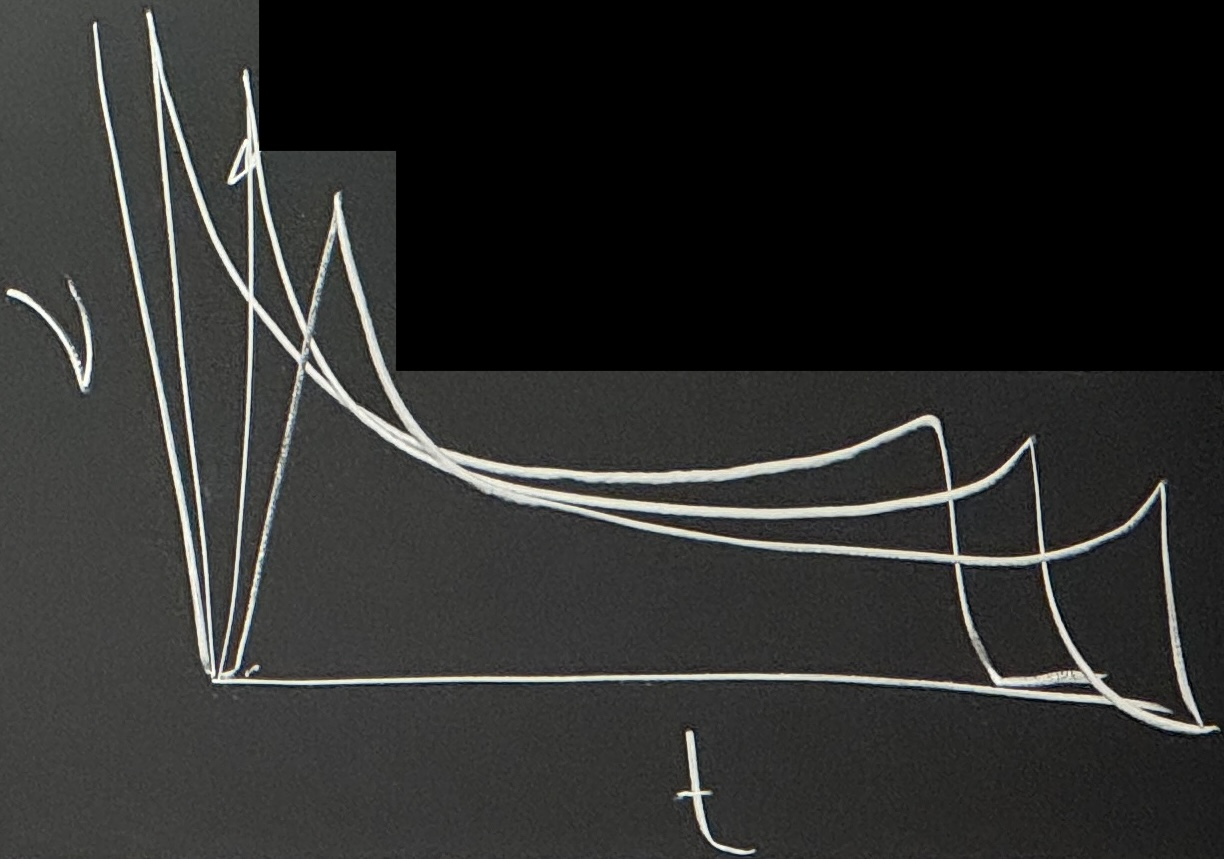
\includegraphics[width=0.8\linewidth]{complexTimecoursea.JPG}
            \caption{The time course.}
            \label{fig:complexTimecoursea}
        \end{subfigure}
        \begin{subfigure}[b]{0.4\linewidth}
            \centering
            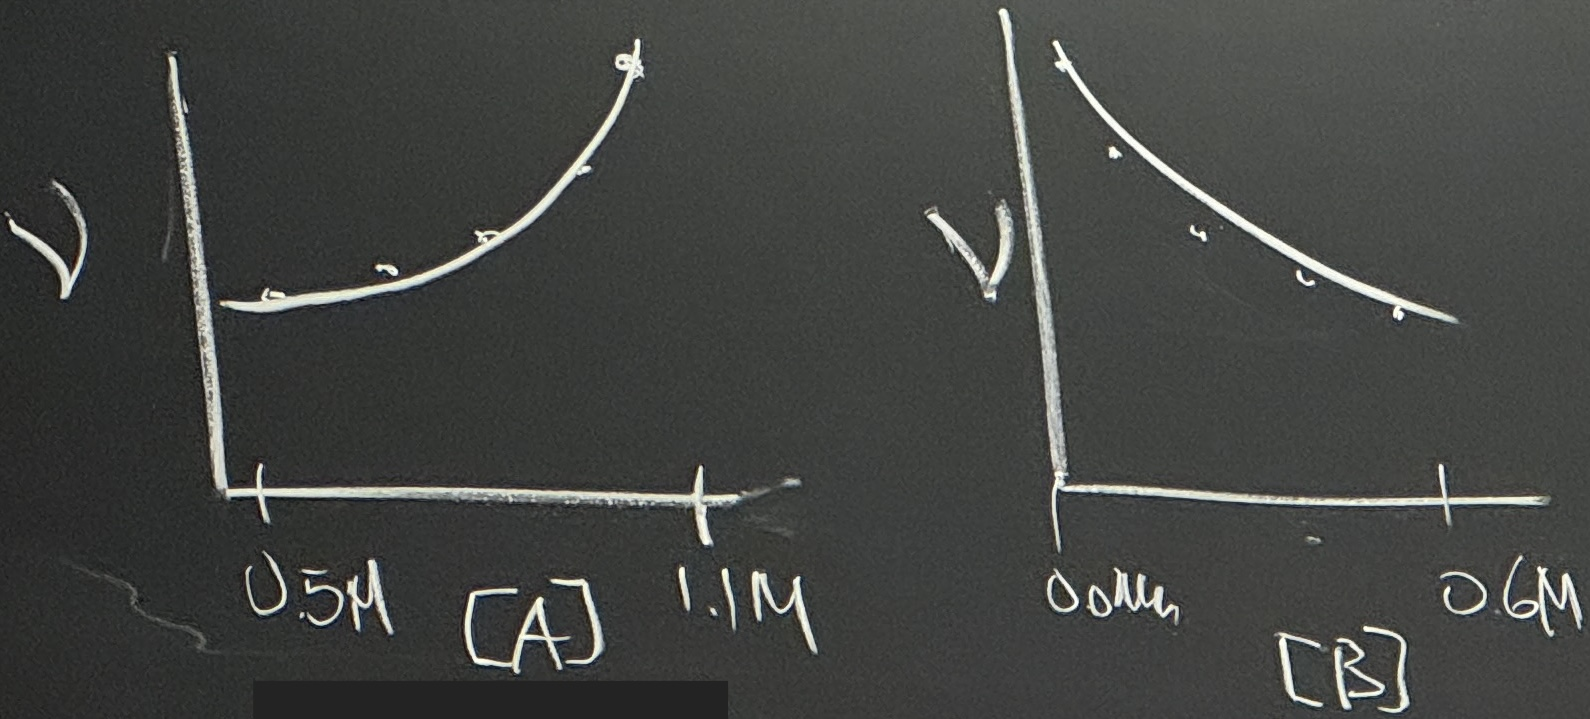
\includegraphics[width=0.9\linewidth]{complexTimecourseb.JPG}
            \caption{The experimental data.}
            \label{fig:complexTimecourseb}
        \end{subfigure}
        \caption{A complex time course.}
        \label{fig:complexTimecourse}
    \end{figure}
    \begin{itemize}
        \item This paper blew Alex's hair back when he read it.
        \item The reaction is nominally pretty straightforward: Aldehyde plus azodicarboxylate in the presence of a chiral prolinate anion organocatalyst, stereoselectively yielding an $\alpha$-amination product.
        \begin{center}
            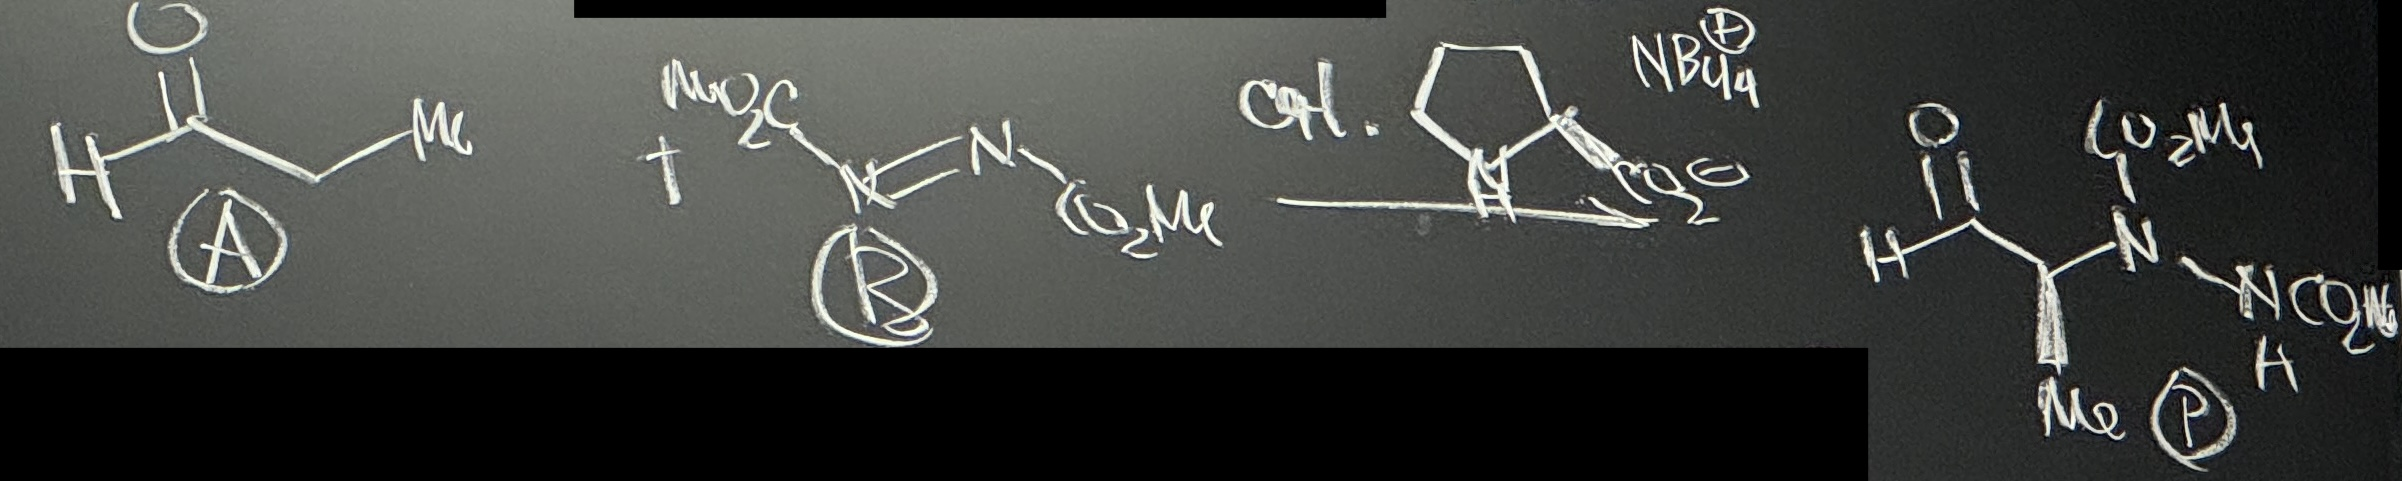
\includegraphics[width=0.7\linewidth]{complexTimecourseRxn.JPG}
        \end{center}
        \begin{itemize}
            \item This is literally the same type of reaction as in Figure \ref{fig:modelCat2Kin}.
        \end{itemize}
        \item The rate was measured via calorimetry in a relevant concentration domain (we didn't have to do weird flooding as with Figure \ref{fig:kAB2}).
        \item Result: We have a complex positive order in $\cnc{A}$, and a complex \emph{inverse} order in $\cnc{B}$ (i.e., at higher concentrations of \ce{B}, the reaction goes slower).
        \item The time course (rate vs. time) is fast acceleration, then slowing down, then speeding up, then dead.
        \begin{itemize}
            \item Here, the full rate course data is \emph{essential} to figuring out what's going on. We would be so wrong it's not even funny if we tried to do method of initial rates here!
            \item As an experimentalist, Alex would first think that his calorimeter is horribly broken. But this is rigorous at different concentrations; this \emph{is} the kinetics!
        \end{itemize}
        \item You can simulate time courses using software packages like COPASI.
    \end{itemize}
    \item The full mechanism that Blackmond and colleagues ended up determining.
    \begin{figure}[H]
        \centering
        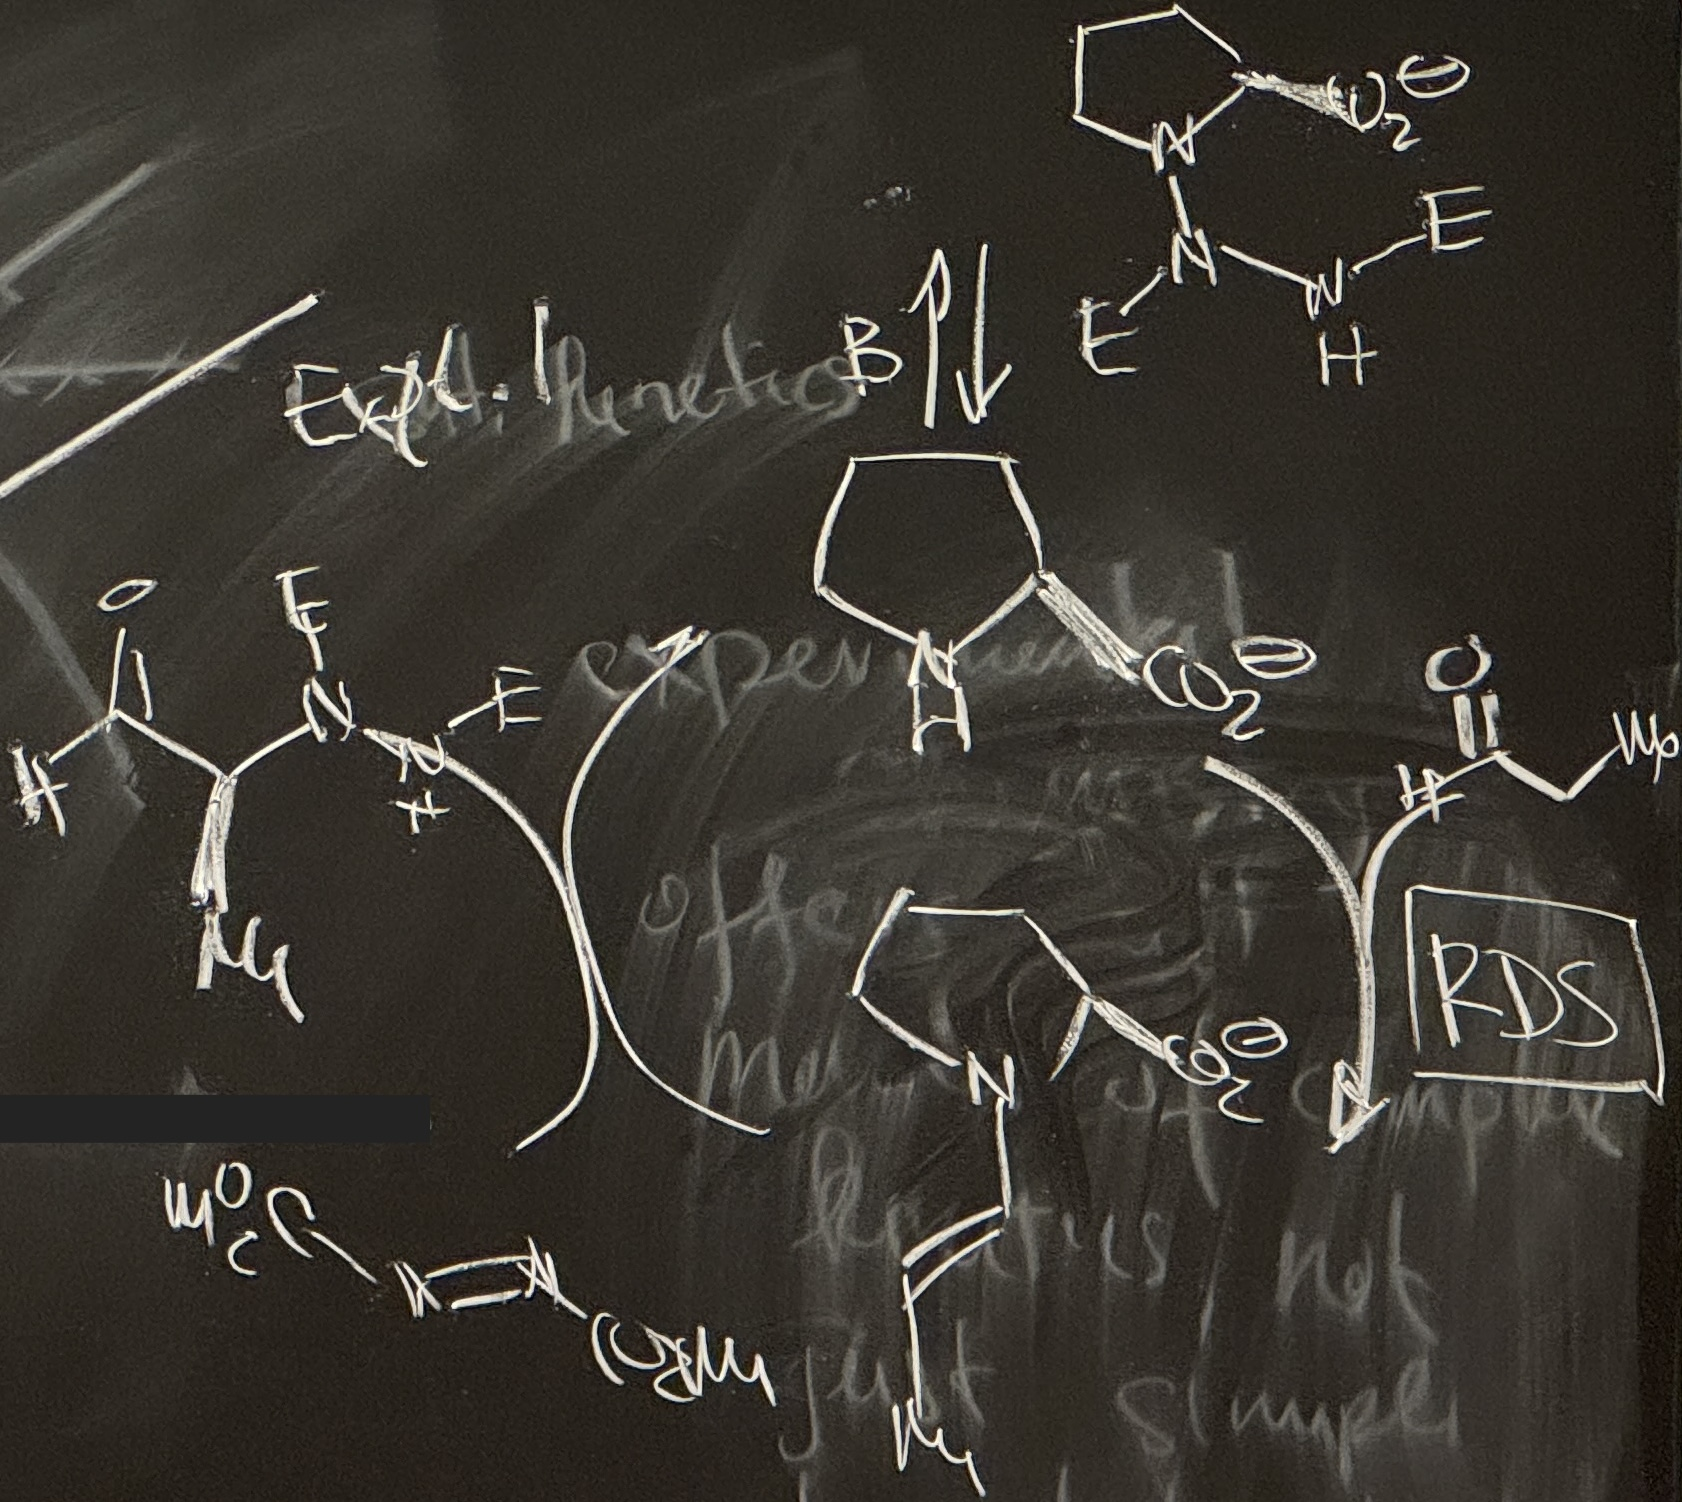
\includegraphics[width=0.4\linewidth]{complexTimecourseMech.JPG}
        \caption{Mechanism underlying an example complex time course.}
        \label{fig:complexTimecourseMech}
    \end{figure}
    \begin{itemize}
        \item This involves an off-cycle equilibrium of the catalyst being sequestered by one of the reagents.
        \item Formation of the enamine is rate-determining.
        \item How important is this whole paper? Alex doesn't know. The beauty of the process may be lost on you if you're a synthetic organic chemist and only care about getting the product.
    \end{itemize}
    \item Challenges with RPKA: Measuring rates directly is difficult, and converting concentration data to rate data propagates some error.
    \item Spiritual successor to RPKA: Variable time normalization analysis (VTNA).
    \begin{figure}[h!]
        \centering
        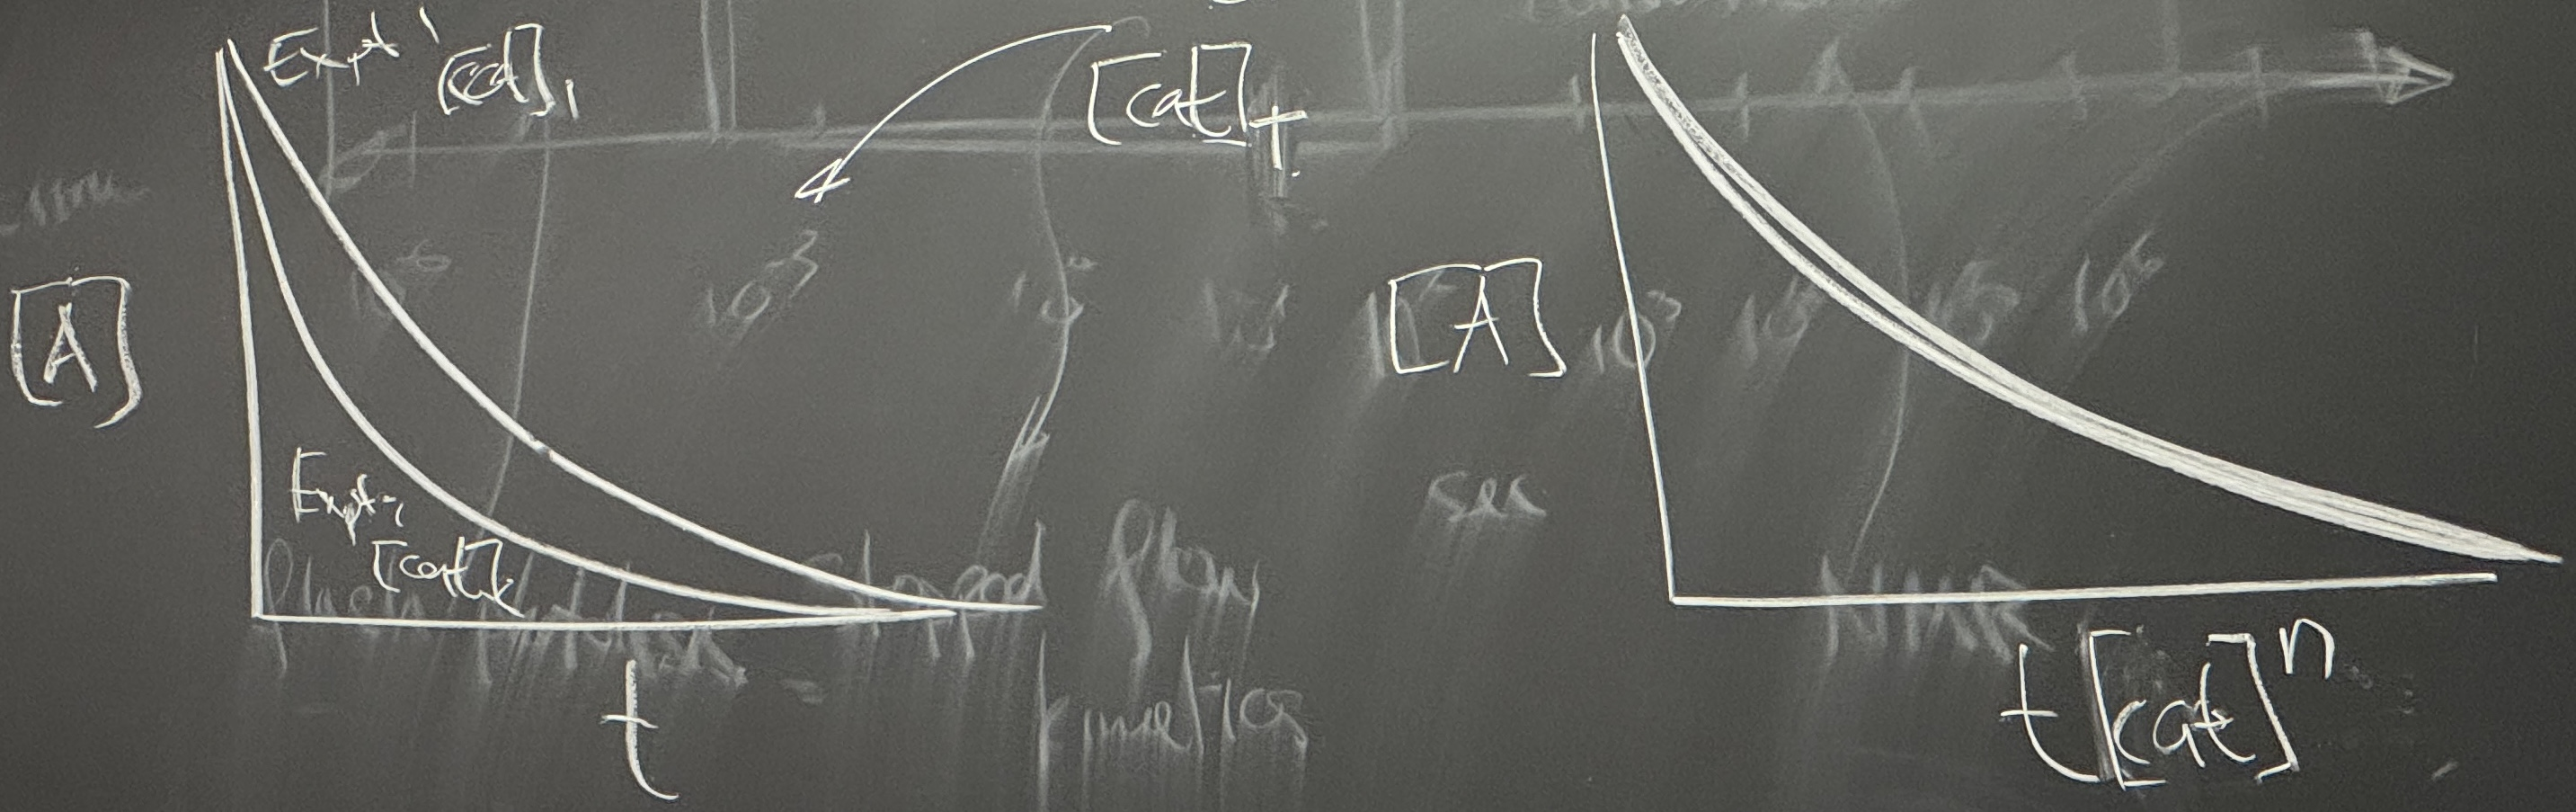
\includegraphics[width=0.7\linewidth]{VTNA.JPG}
        \caption{Variable time normalization analysis.}
        \label{fig:VTNA}
    \end{figure}
    \begin{itemize}
        \item Reference: Work by Jordi Bur\'{e}s.
        \begin{itemize}
            \item Initial set of papers: \textcite{bib:VTNA1}.
            \item A really useful tutorial: \textcite{bib:VTNA2}.
        \end{itemize}
        \item Collect concentration vs. time data (e.g., via GC-MS aliquots as per usual).
        \item Change the total catalyst concentration $\cnc[T]{cat}$ and look how the rates change.
        \item Key insight: $\cnc[T]{cat}$ is basically constant during the reaction, so just treat it as a parameter of the system.
        \item Normalize to $\cnc{cat}^n$ by varying $n$ until you get overlay and call that the order!
    \end{itemize}
    \pagebreak
    \item Using VTNA, you can also normalize not only to something that's constant, but to something that's variable.
    \begin{figure}[h!]
        \centering
        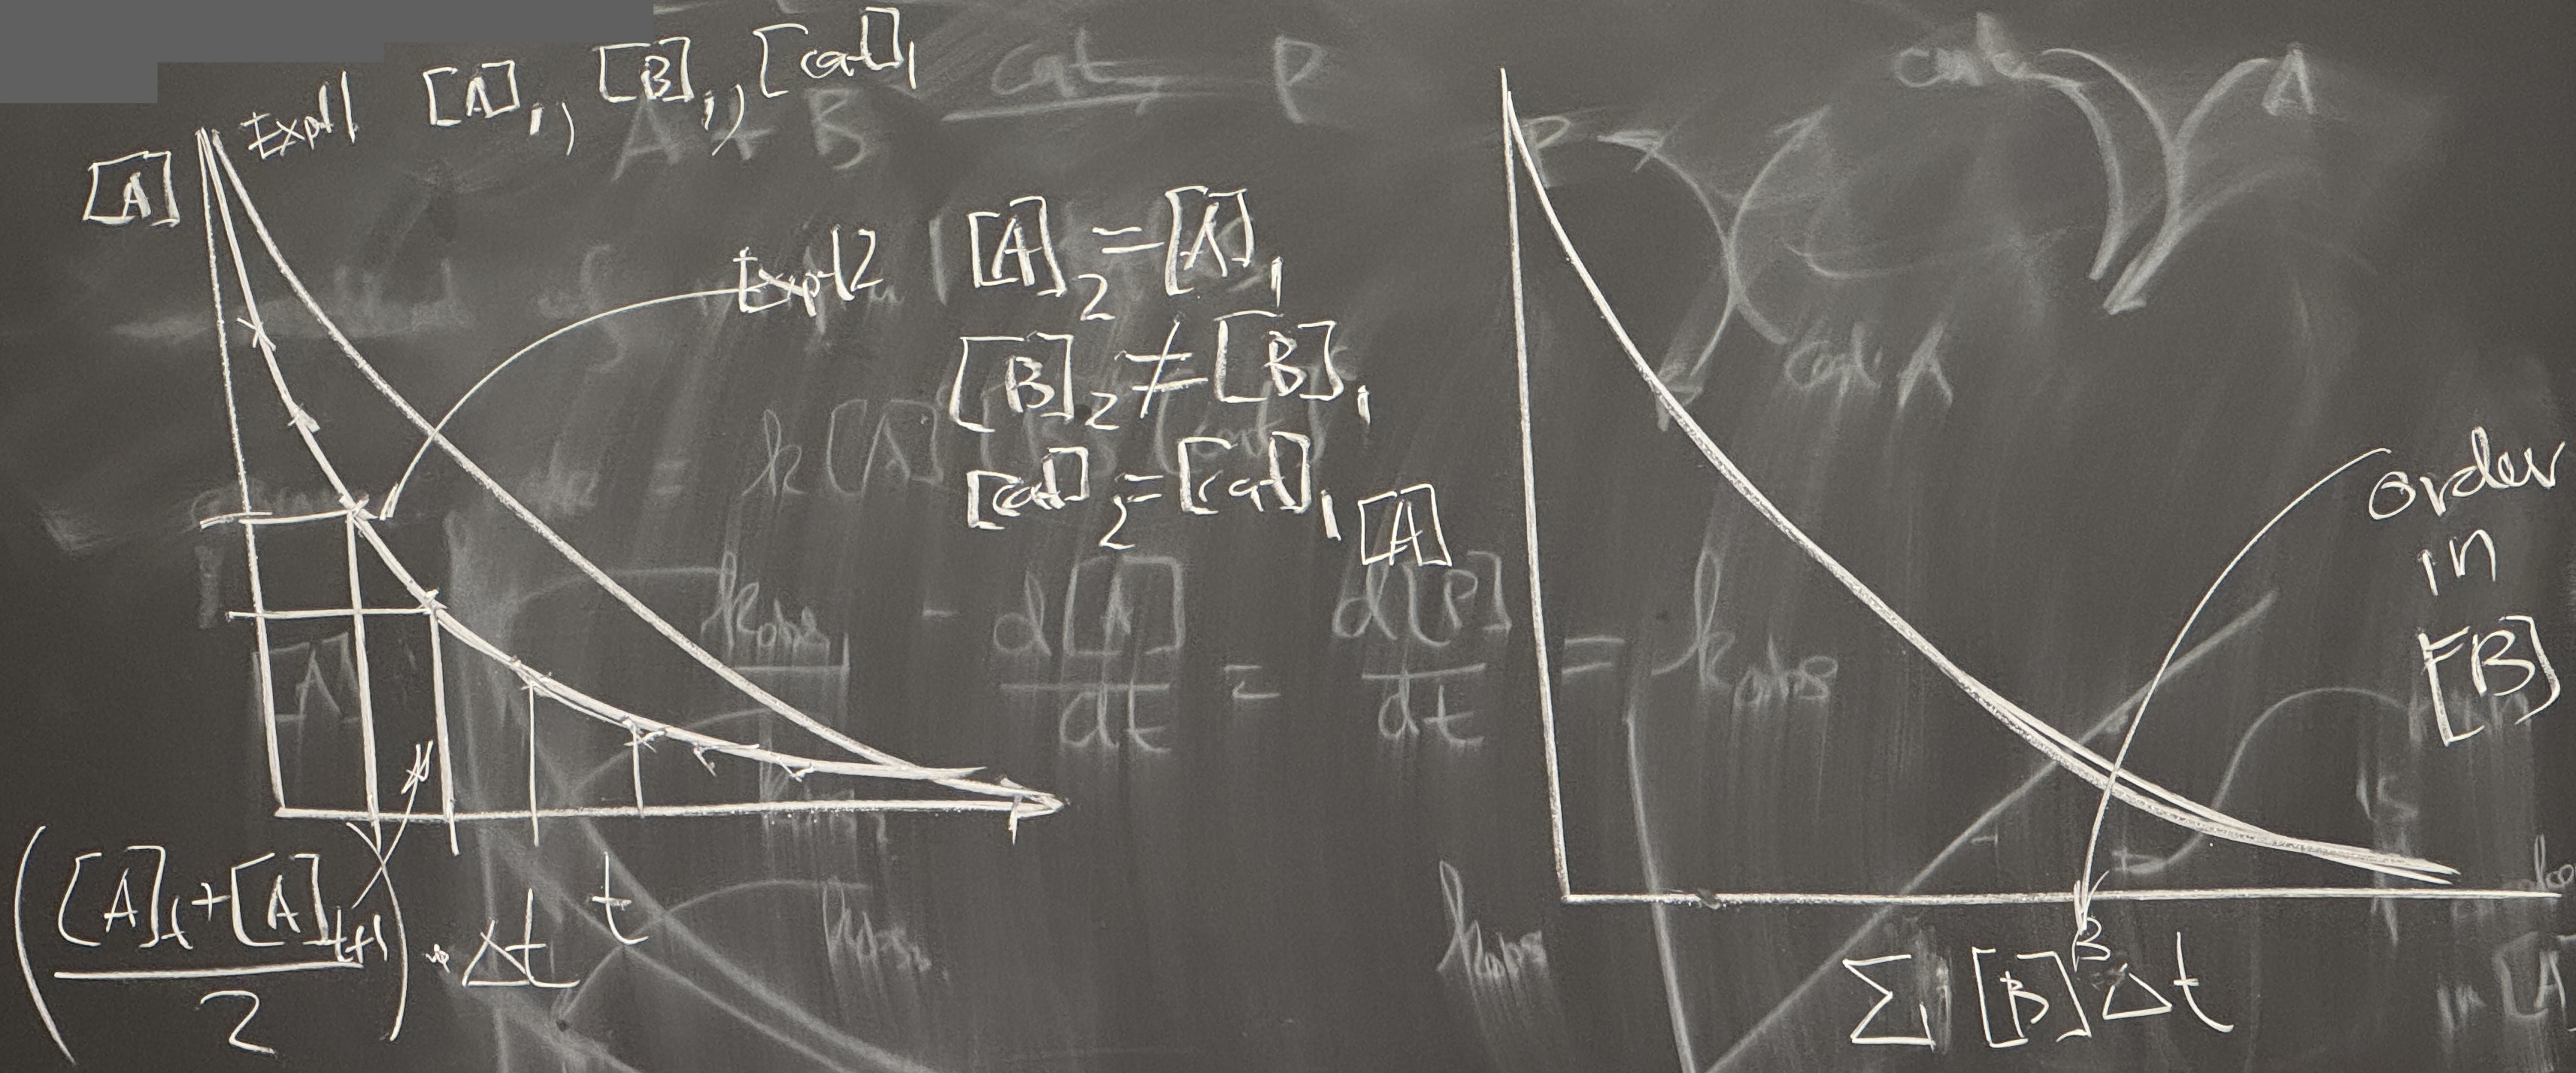
\includegraphics[width=0.7\linewidth]{VTNAdiffExcess.JPG}
        \caption{Variable time normalization analysis (different excess experiment).}
        \label{fig:VTNAdiffExcess}
    \end{figure}
    \begin{itemize}
        \item Do a different excess experiment.
        \item Experiment 1: Run it with $\cnc[1]{A}$, $\cnc[1]{B}$, and $\cnc[1]{cat}$.
        \item Experiment 2: Keep $\cnc[2]{A}=\cnc[1]{A}$ and $\cnc[2]{cat}=\cnc[1]{cat}$, but change $\cnc[2]{B}\neq\cnc[1]{B}$.
        \item $\cnc{B}$ is being consumed during the reaction, so it's changing in a stoichiometric fashion.
        \item Use the trapezoid rule to integrate under the Experiment 2 curve. Then plot $\cnc{A}$ vs. our new time-normalized $x$-axis, and vary $\beta$ until we get the correct reaction order.
    \end{itemize}
\end{itemize}




\end{document}